% Chương 2: Thực nghiệm và đánh giá.
% Hình lấy từ results/figures/ (\graphicspath trong report.tex), bảng từ tables/*.tex.
% Cả hình và bảng do scripts/make_figures.jl sinh từ các CSV trong results/; số liệu trong bài lấy từ chính các bảng đó.

\section{\texorpdfstring{Thực nghiệm và đánh giá}{CHƯƠNG 2: THỰC NGHIỆM VÀ ĐÁNH GIÁ}}
\label{sec:experiments}

Chương này so sánh cài đặt FPClose của nhóm với cài đặt FPClose trong thư viện SPMF~\cite{spmf} trên chín CSDL
benchmark theo sáu tiêu chí: tính đúng đắn (\textit{correctness}), thời gian chạy theo ngưỡng hỗ trợ tối thiểu
(\textit{minimum support}, minsup), số itemset sinh ra, bộ nhớ, khả năng mở rộng (\textit{scalability}) và ảnh hưởng
của độ dài giao dịch. Mục~\ref{sec:setup} mô tả thiết lập thực nghiệm, các mục tiếp theo trình bày lần lượt từng tiêu
chí, hai mục cuối phân tích độ phức tạp và tổng kết.

\subsection{Thiết lập thực nghiệm}
\label{sec:setup}

\textbf{Dữ liệu.} Nhóm dùng chín cơ sở dữ liệu (CSDL) giao dịch phổ biến trong cộng đồng khai thác tập phổ biến
(\textit{Frequent Itemset Mining}, FIM), lấy từ SPMF và kho FIMI~\cite{fimi03} (Bảng~\ref{tab:datasets}). Mỗi file
được chuẩn hóa về định dạng SPMF (mỗi dòng một giao dịch, item là số nguyên dương sắp tăng, không trùng) và lưu công
khai trên Hugging Face (\url{https://huggingface.co/datasets/hytrang/fpclose-fim-benchmarks}) kèm SHA-256 của từng
file. Riêng mushrooms dùng bản FIMI gồm 8\,124 giao dịch, khớp số mẫu của bộ UCI Mushroom~\cite{uci_mushroom}. Chi
tiết chuẩn hóa nằm ở Phụ lục~\ref{app:data}. Mật độ trong Bảng~\ref{tab:datasets} là mật độ toàn cục
\begin{equation}
\operatorname{Density}(D)=\frac{\sum_{i=1}^{n}|T_i|}{n\,|I|}\times 100\%=\frac{\bar{w}}{|I|}\times 100\%,
\label{eq:density}
\end{equation}
với $n$ là số giao dịch, $T_i$ là giao dịch thứ $i$, $\bar{w}$ là độ dài giao dịch trung bình và $I$ là tập các item
phân biệt trước khi lọc theo minsup. Mật độ toàn cục là trung bình độ hỗ trợ tương đối của các item, tính theo phần
trăm. Trong phạm vi thực nghiệm này, chín CSDL được phân nhóm quy ước thành \textbf{dày} (\textit{dense}: chess,
mushrooms, connect, pumsb\_star, accidents) và \textbf{thưa} (\textit{sparse}: retail, T10I4D100K, T40I10D100K,
kosarak). Bài báo gốc cũng xếp connect và accidents vào dữ liệu dày~\cite{grahne2005}. Mật độ không phải tiêu chí
phân nhóm duy nhất: tỉ lệ kích thước FP-tree tại minsup giữa lưới, định nghĩa ở (\ref{eq:tree-ratio}), là
0{,}03--10{,}56\% ở nhóm dày và 28{,}14--89{,}13\% ở nhóm thưa (Bảng~\ref{tab:fptree}), hỗ trợ cách phân nhóm này.

\textbf{Lưới minsup.} Với mỗi CSDL, nhóm chạy thử SPMF trên nhiều mức minsup với giới hạn 300\,s mỗi lần chạy và giữ
6–7 mức từ cao xuống thấp mà SPMF chạy xong, tổng cộng 56 cấu hình. Ba mức thấp hơn bị loại vì SPMF vượt giới hạn
này (kosarak 0{,}15\% và 0{,}1\%, T40I10D100K 0{,}5\%). Ngưỡng tương đối được đổi sang số giao dịch bằng
$\sigma = \lceil n \cdot \text{minsup} \rceil$, giống SPMF. Trong lần đo chính, mỗi lần chạy có giới hạn 600\,s và
không lần chạy nào vượt giới hạn.

\begin{table}[!htb]
\caption{Chín CSDL benchmark sau khi chuẩn hóa}
\label{tab:datasets}
\centering
\fittable{\columnwidth}{datasets_table}
\end{table}

\textbf{Cách đo.} Mọi phép đo chạy trên cùng một máy (AMD Ryzen~9 8940HX, 16\,GB RAM, Windows, Julia 1.13.4, OpenJDK
25, SPMF với \texttt{-Xmx4g}), quy trình đo được tự động hóa và tái lập được (Phụ lục~\ref{app:repro}). Thời gian của
nhóm gồm đọc file, khai thác và ghi kết quả. Thời gian của SPMF là ``Total time'' do SPMF tự in: theo mã của lớp
\texttt{AlgoFPClose}, đồng hồ bắt đầu khi gọi thuật toán và dừng sau khi đóng file kết quả, nên cũng gồm đọc, khai
thác và ghi, với độ phân giải mili giây. Thời gian khởi động JVM và Julia không được tính ở cả hai phía. Hai phía
khác nhau ở bước warm-up: mỗi lần đo của nhóm chạy trong một tiến trình Julia riêng, có \textit{warm-up} trên một
CSDL nhỏ để loại phần lớn thời gian biên dịch JIT, còn mỗi lần chạy SPMF dùng một JVM mới không warm-up, nên thời
gian biên dịch JIT của JVM nằm trong Total time. Phép so vì vậy phản ánh hiệu năng của hai cài đặt trong điều kiện
thực thi này, và lợi thế của nhóm ở các cấu hình chạy rất nhanh có thể bị phóng đại. Bộ nhớ của nhóm là RSS đỉnh
(\textit{resident set size}: bộ nhớ vật lý tiến trình chiếm) đọc bằng \texttt{Sys.maxrss}, gồm khoảng 285\,MB nền của
Julia. ``Max memory'' của SPMF là heap JVM, đo theo cách khác, nên bộ nhớ chỉ được so giữa các biến thể của nhóm.

\textbf{Tổng hợp số đo.} Mỗi cấu hình được đo ba lần. Khi so thời gian với SPMF, nhóm báo cáo giá trị nhỏ nhất, tức
thời gian thực thi tốt nhất quan sát được (\textit{best observed runtime}), theo phương pháp của Chen và
Revels~\cite{chen2016}. Thực nghiệm bộ nhớ và ablation dùng trung vị. Với $r = T_{\text{nhóm}}/T_{\text{SPMF}}$, nhóm
quy ước $r<0{,}90$ là nhanh hơn, $0{,}90 \le r \le 1{,}10$ là gần tương đương và $r>1{,}10$ là chậm hơn, dựa trên
mức biến thiên giữa các lần đo. Đây là ngưỡng sai khác thực tiễn, không phải ngưỡng ý nghĩa thống kê. Phân tích độ
nhạy trên 78 cấu hình so sánh cho thấy không cấu hình nào đảo chiều nhanh/chậm và 74/78 cấu hình giữ nguyên nhóm khi
dùng trung vị thay giá trị nhỏ nhất (Phụ lục~\ref{app:data}).

% ---------------------------------------------------------------------------
\subsection{Tính đúng đắn}
\label{sec:correctness}

Với mỗi cấu hình, kết quả của hai phía được đưa về tập các cặp (itemset, support) rồi so trực tiếp. Tỉ lệ khớp được
tính là
\begin{equation}
  \text{match} = \frac{|M|}{|M| + |O_{\text{nhóm}}| + |O_{\text{SPMF}}| + |D|},
\end{equation}
trong đó $M$ là các itemset có ở cả hai phía với cùng support, $O_{\text{nhóm}}$ và $O_{\text{SPMF}}$ là các itemset
chỉ một phía có, $D$ là các itemset có ở cả hai phía nhưng khác support. Mẫu số là số itemset khác nhau của cả hai
phía, nên itemset thừa ở phía nhóm cũng bị tính là sai.

Bảng~\ref{tab:correctness} cho thấy cài đặt của nhóm khớp hoàn toàn với SPMF về \textit{closed itemset} và support
trên cả 56 cấu hình, với tổng cộng 848\,998 lượt kết quả được đối chiếu qua các cấu hình. Khả năng khôi phục mọi
\textit{frequent itemset} từ tập đóng cũng khớp với \texttt{FPGrowth\_itemsets} của SPMF tại 9 cấu hình, mỗi CSDL một
mức minsup cao nhất, vì số frequent itemset bùng nổ khi minsup giảm (mushrooms 20\% đã có 53\,583 frequent itemset so
với 1\,197 tập đóng). Bản thân SPMF cũng được kiểm tra trước khi dùng làm đáp án: trên cả 56 cấu hình, kết quả của
SPMF giống từng itemset và support với cài đặt FPclose gốc của các tác giả trong kho FIMI~\cite{grahne2003}.

\begin{table*}[!t]
\caption{Tỉ lệ itemset khớp SPMF (closed: mọi cấu hình, mọi frequent itemset: minsup cao nhất)}
\label{tab:correctness}
\centering
\fittable{\textwidth}{correctness_table}
\end{table*}

Kết quả cuối không còn sai lệch. Sai khác phát hiện trước đó liên quan đến phép chuyển minsup tương đối sang số giao
dịch bằng số thực dấu phẩy động: tích $0{,}07 \times 100$ được biểu diễn là $7{,}000000000000001$ nên hàm làm tròn lên
trả về 8, dù theo số học chính xác ngưỡng là 7. Nhóm áp dụng quy ước tương thích SPMF trong phép đối chiếu. Các chi
tiết triển khai khác phát hiện khi kiểm thử được trình bày ở Mục~\ref{sec:deviations}.

% ---------------------------------------------------------------------------
\subsection{Thời gian chạy theo minsup}
\label{sec:runtime}

Hình~\ref{fig:rt-chess}–\ref{fig:rt-kosarak} vẽ thời gian của nhóm và SPMF trên từng CSDL, mỗi hình một CSDL như
cách trình bày của bài báo gốc~\cite{grahne2005}: trục hoành là các mức minsup rời rạc giảm dần từ trái sang phải,
trục tung thang log. Tỉ lệ thời gian nhóm/SPMF tại từng mức minsup nằm ở Bảng~\ref{tab:ratio} (Phụ lục) và được diễn
giải theo ngưỡng ở Mục~\ref{sec:setup}.

\colfig{runtime_chess.pdf}{Thời gian chạy trên chess.}{fig:rt-chess}
\colfig{runtime_mushrooms.pdf}{Thời gian chạy trên mushrooms.}{fig:rt-mushrooms}
\colfig{runtime_connect.pdf}{Thời gian chạy trên connect.}{fig:rt-connect}
\colfig{runtime_pumsb_star.pdf}{Thời gian chạy trên pumsb\_star.}{fig:rt-pumsb_star}
\colfig{runtime_accidents.pdf}{Thời gian chạy trên accidents.}{fig:rt-accidents}

\textbf{CSDL nhóm có lợi thế.} Nhóm nhanh hơn SPMF trên chess (tỉ lệ 0{,}11–0{,}56) và mushrooms (0{,}43–0{,}62), và
khoảng cách tăng khi minsup giảm: ở chess 60\%, thời gian tốt nhất quan sát được của nhóm là 0{,}85\,s so với
7{,}85\,s của SPMF. Trên connect, nhóm chậm hơn ở minsup cao (1{,}87), gần tương đương ở 75\% (0{,}92) và nhanh hơn ở
70\% (0{,}66).

\colfig{runtime_retail.pdf}{Thời gian chạy trên retail.}{fig:rt-retail}
\colfig{runtime_T10I4D100K.pdf}{Thời gian chạy trên T10I4D100K.}{fig:rt-T10I4D100K}
\colfig{runtime_T40I10D100K.pdf}{Thời gian chạy trên T40I10D100K.}{fig:rt-T40I10D100K}
\colfig{runtime_kosarak.pdf}{Thời gian chạy trên kosarak.}{fig:rt-kosarak}

\textbf{Các CSDL còn lại.} Nhóm chậm hơn trên accidents (1{,}74–2{,}48), pumsb\_star (1{,}23–1{,}67), kosarak
(1{,}17–2{,}60) và T10I4D100K (1{,}19–1{,}67) ở mọi mức khảo sát. Retail (0{,}92–1{,}57) và T40I10D100K
(0{,}98–1{,}33) gần tương đương ở một vài mức minsup cao và chậm hơn ở minsup thấp. Một số cấu hình có khoảng đo của
hai phía chồng lấn nhau nên cần diễn giải thận trọng (Phụ lục~\ref{app:data}).

\textbf{Giải thích theo thuật toán.} Theo cơ chế FP-tree và CFI-tree của FPClose~\cite{grahne2005}, chi phí khai thác
phụ thuộc vào mức chia sẻ tiền tố của cây, kích thước pattern base và cây điều kiện, cùng chi phí kiểm tra tính đóng
(Mục~\ref{sec:complexity}). Kích thước đầu ra có liên quan nhưng không xác định duy nhất thời gian chạy. Trên chess
60\%, số tập đóng lớn (98\,392) và bước khai thác chiếm 0{,}75 trong 0{,}85\,s, đây là vùng cài đặt của nhóm có lợi
thế. Ngược lại, tỉ lệ kích thước FP-tree $R_{\text{tree}}$ (số nút FP-tree gốc chia cho tổng lượt item phổ biến, công
thức~(\ref{eq:tree-ratio})) ở dữ liệu thưa cao hơn hẳn dữ liệu dày (Bảng~\ref{tab:fptree}). Khi cây gần to bằng dữ
liệu, phần xử lý từng giao dịch (đọc, sắp xếp, chèn) chiếm tỉ trọng lớn hơn. Phân rã thời gian
(Bảng~\ref{tab:breakdown}) cho thấy bước đọc file chiếm phần đáng kể trong cài đặt của nhóm, khoảng 1{,}1\,s trên
accidents 40\% (30\% tổng thời gian) và kosarak 0{,}2\% (19\%). Vì chưa có phân rã tương ứng của SPMF, nhóm chưa định
lượng được phần đóng góp của từng bước vào chênh lệch giữa hai cài đặt.

% ---------------------------------------------------------------------------
\subsection{Số lượng itemset theo minsup}
\label{sec:itemsets}

Hình~\ref{fig:it-dense} và~\ref{fig:it-sparse} vẽ số closed frequent itemset theo minsup (cả hai trục thang log, trục
hoành là minsup thật nên mỗi CSDL nằm ở một khoảng riêng).

\colfig{itemsets_dense.pdf}{Số closed itemset theo minsup trên dữ liệu dày.}{fig:it-dense}
\colfig{itemsets_sparse.pdf}{Số closed itemset theo minsup trên dữ liệu thưa.}{fig:it-sparse}

Khi minsup giảm, số tập đóng tăng nhanh ở cả hai nhóm, nhưng ở hai vùng minsup rất khác nhau. Chess tăng từ 498 tập
tại minsup 90\% lên 98\,392 tập tại 60\%, accidents từ 31 (90\%) lên 32\,528 (40\%). Retail tăng từ 159 tập tại 1\%
lên 65\,301 tập tại 0{,}02\%, T10I4D100K từ 385 lên 107\,822. Các CSDL dày được khảo sát vì vậy phát sinh đầu ra lớn
ngay ở ngưỡng hỗ trợ cao, do nhiều item cùng xuất hiện trong phần lớn giao dịch, còn các CSDL thưa cần minsup thấp
hơn hai bậc độ lớn. Mức đồng xuất hiện của item và cấu trúc giao dịch ảnh hưởng đến không gian khai thác. Kích thước
đầu ra có liên quan đến thời gian chạy nhưng không phải yếu tố duy nhất, vì thời gian còn phụ thuộc cấu trúc cây và
hiệu quả cắt nhánh. Lưới minsup vì vậy được chọn riêng cho từng CSDL (60–95\% cho chess và connect, 0{,}02–1\% cho
retail và T10I4D100K).

% ---------------------------------------------------------------------------
\subsection{Sử dụng bộ nhớ: bản cơ bản và bản tối ưu}
\label{sec:memory}

Thực nghiệm chạy ba biến thể của cùng cài đặt ở mức minsup giữa lưới của mỗi CSDL: \textbf{cơ bản} (tắt mọi tối
ưu), \textbf{chỉ cắt nhánh} (chỉ bật cắt nhánh ở dòng 8 của mã giả FPClose) và \textbf{tối ưu} (bật cắt nhánh,
FP-array, kết thúc sớm, so count chính xác và CFI-tree rút gọn). FP-array là mảng đếm sẵn tần suất của từng cặp item
khi dựng cây, nhờ đó khi dựng cây điều kiện không phải duyệt cây thêm một lần để đếm~\cite{grahne2005}. Cả ba biến
thể cho cùng một tập kết quả ở mọi lần chạy (cùng mã hash). RAM tối đa và thời gian khai thác là trung vị của ba lần
đo (Hình~\ref{fig:memory}, số liệu ở Bảng~\ref{tab:memory}, Phụ lục).

\begin{figure*}[!t]
\centering
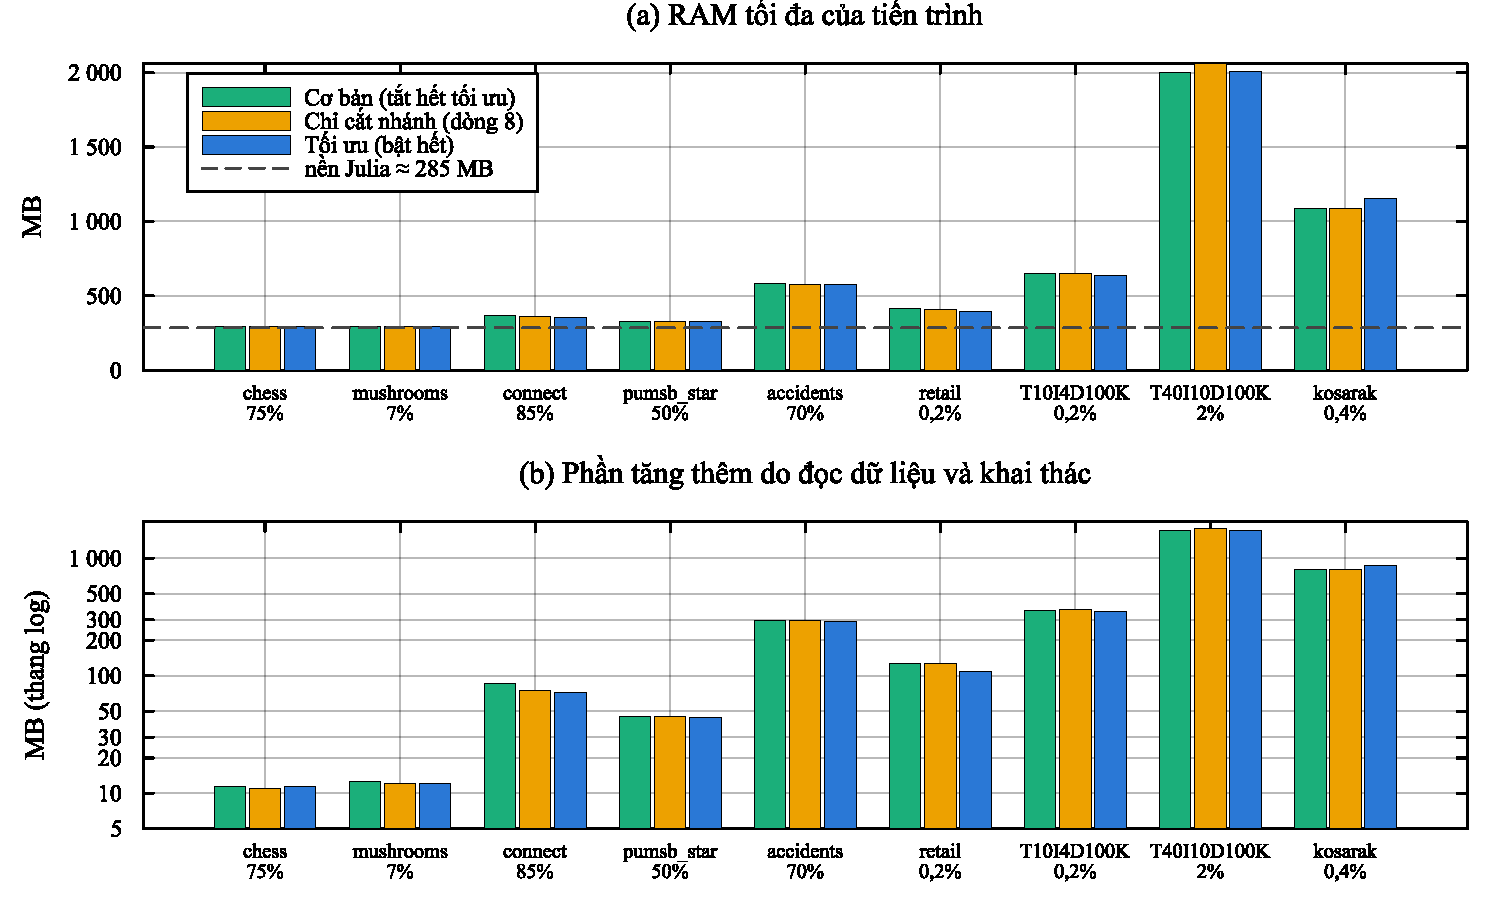
\includegraphics[width=\textwidth]{memory_basic_vs_optimized.pdf}
\caption{Bộ nhớ của ba biến thể tại minsup giữa lưới: (a) RAM tối đa của tiến trình (gồm khoảng 285\,MB nền của Julia),
(b) RAM tối đa tăng thêm so với mốc sau warm-up (\textit{incremental peak RSS}), thang log. Trung vị của 3 lần đo.}
\label{fig:memory}
\end{figure*}

\textbf{RAM tối đa.} Phần tăng thêm so với mốc sau warm-up đi từ khoảng 11\,MB trên chess đến khoảng 1{,}7\,GB trên
T40I10D100K và 0{,}8\,GB trên kosarak. Đây không phải bộ nhớ riêng của thuật toán mà gồm CSDL nạp vào bộ nhớ, FP-tree
gốc và các cây điều kiện đang mở trên đường đệ quy. T40I10D100K cần nhiều nhất vì FP-tree gốc gần như không nén được
(khoảng 3{,}26 triệu nút, $R_{\text{tree}}=89\%$) và giao dịch dài (trung bình 39{,}6 item).

\textbf{Bản tối ưu so với bản cơ bản.} Bản tối ưu giảm RAM tối đa trên connect (371 xuống 356\,MB), retail (414
xuống 399\,MB) và T10I4D100K (649 xuống 638\,MB), chênh lệch trên các CSDL còn lại khá nhỏ. Ngược lại, trên kosarak
RAM tối đa tăng từ 1\,089 lên 1\,153\,MB, khi tắt riêng FP-array thì còn 1\,101\,MB, cho thấy FP-array có thể làm
tăng chi phí bộ nhớ. Về thời gian khai thác, tỉ lệ bản cơ bản/bản tối ưu đi từ 0{,}98 trên accidents (bản cơ bản đo
được hơi nhanh hơn, trong phạm vi nhiễu) đến 1{,}32 trên mushrooms, tức bản tối ưu giảm khoảng 24\% thời gian khai
thác trên mushrooms. Phép thử loại bỏ (\textit{ablation}, Bảng~\ref{tab:ablation}, Phụ lục) tắt riêng từng tối ưu
và cho thấy lợi ích phụ thuộc CSDL:
\begin{itemize}
  \item Tắt \textbf{FP-array} làm thời gian khai thác tăng 28\% trên T40I10D100K và 18\% trên T10I4D100K. FP-array
        chỉ được dùng trên dữ liệu thưa (941 lần trên retail, 0 lần trên mọi CSDL dày) vì nó được tắt khi cây đủ dày,
        đúng như bài báo đề xuất~\cite{grahne2005}.
  \item \textbf{Cắt nhánh} và \textbf{kết thúc sớm} giảm số lời gọi đệ quy trên dữ liệu dày (mushrooms từ 15\,095
        xuống 8\,158, connect từ 13\,362 xuống 8\,212) và gần như không kích hoạt trên dữ liệu thưa.
  \item Tắt \textbf{CFI-tree rút gọn} làm thời gian khai thác tăng 13–16\% trên chess và mushrooms.
\end{itemize}
Các chênh lệch dưới khoảng 10\% được diễn giải thận trọng vì chỉ có ba lần đo. Chạy lại toàn bộ thực nghiệm bộ nhớ
trên một máy khác cho cùng tập kết quả ở cả 216 lần chạy, RAM tối đa lệch trung vị 0{,}9\% (Phụ lục~\ref{app:data}).

% ---------------------------------------------------------------------------
\subsection{Khả năng mở rộng}
\label{sec:scalability}

Nhóm dùng retail (88\,162 giao dịch) và tạo năm tập con lồng nhau gồm 10\%, 25\%, 50\%, 75\% và 100\% giao dịch (xáo
trộn một lần với seed cố định rồi lấy tiền tố), ở hai mức minsup tương đối 0{,}1\% và 0{,}05\%. Trong các tập con
này, số tập đóng gần ổn định theo kích thước: 7\,572–8\,394 ở 0{,}1\% và 18\,925–19\,579 ở 0{,}05\%.

\colfig{scalability_time.pdf}{Thời gian theo kích thước CSDL trên các tập con của retail.}{fig:sc-time}

Hình~\ref{fig:sc-time} (số liệu ở Bảng~\ref{tab:scalability} và Hình~\ref{fig:sc-ratio}, Phụ lục) cho thấy khi số
giao dịch tăng 10 lần, thời gian của nhóm tăng 10{,}5 lần ở minsup 0{,}1\% và 7{,}5 lần ở 0{,}05\%. Mô hình tuyến
tính $T(n)=an+b$ khớp tốt cho cả hai cài đặt ($R^2 \geq 0{,}97$), gợi ý xu hướng mở rộng gần tuyến tính trong phạm
vi retail và hai mức minsup khảo sát. Thời gian của SPMF chỉ tăng 3{,}1–3{,}5 lần, hệ số chặn $b$ của SPMF là
0{,}12–0{,}17\,s (22–25\% thời gian ở 100\%) còn của nhóm gần bằng 0. Hệ số chặn dương gợi ý SPMF có một thành phần
chi phí ít phụ thuộc kích thước dữ liệu, nhưng thực nghiệm này không xác định nguồn của chi phí đó. Hệ quả là nhóm
nhanh hơn SPMF trên các tập con nhỏ (0{,}071 so với 0{,}158\,s ở 10\%), gần tương đương ở 75\% với minsup 0{,}1\%
(1{,}09) và chậm hơn trên toàn bộ retail (0{,}75 so với 0{,}55\,s). Điều này nhất quán với Mục~\ref{sec:runtime}:
chi phí xử lý từng giao dịch của nhóm tăng theo khối lượng dữ liệu.

% ---------------------------------------------------------------------------
\subsection{Ảnh hưởng của độ dài giao dịch trung bình}
\label{sec:txlen}

Giao dịch dài có thể làm tăng độ sâu FP-tree, kích thước pattern base và số tổ hợp item cần khảo sát. Để kiểm
chứng, nhóm sinh sáu CSDL tổng hợp cùng 10\,000 giao dịch, miền 500 item, độ dài trung bình 5, 10, \ldots, 30. Giao
dịch của mức dài chứa giao dịch của mức ngắn, quy trình sinh nằm ở Phụ lục~\ref{app:data}. Vì miền item được giữ cố
định, khi độ dài tăng thì mật độ và mức đồng xuất hiện của item cũng thay đổi theo. Nhóm chạy ở hai mức minsup
0{,}5\% và 0{,}2\%.

\colfig{txlen_time.pdf}{Thời gian theo độ dài giao dịch trung bình (10\,000 giao dịch, 500 item).}{fig:tx-time}
\colfig{txlen_itemsets.pdf}{Số closed itemset theo độ dài giao dịch trung bình (10\,000 giao dịch, 500 item).}{fig:tx-items}

Hình~\ref{fig:tx-time} và~\ref{fig:tx-items} (số liệu ở Bảng~\ref{tab:txlen}, Phụ lục) cho thấy khi độ dài trung
bình tăng từ 5 lên 30, số tập đóng tăng khoảng 38 lần (470 lên 18\,038) ở minsup 0{,}5\% và 160 lần (914 lên
146\,134) ở 0{,}2\%, thời gian của nhóm tăng tương ứng khoảng 29 lần (0{,}017 lên 0{,}49\,s) và 98 lần (0{,}019 lên
1{,}89\,s). Thời gian và số tập đóng tăng nhanh trong khoảng độ dài 5–30, nhưng sáu điểm đo không đủ để khẳng định một
quy luật hàm mũ. Nhóm nhanh hơn hoặc gần tương đương SPMF ở mọi cấu hình khảo sát (tỉ lệ 0{,}34 ở độ dài 5,
0{,}76–0{,}82 ở độ dài 30). Tại minsup 0{,}2\% và độ dài 20, 25, tỉ lệ là 0{,}93 và 0{,}98, tức gần tương đương. Nhìn
chung lợi thế của nhóm thu hẹp khi giao dịch dài ra.

% ---------------------------------------------------------------------------
\subsection{Phân tích độ phức tạp}
\label{sec:complexity}

Gọi $n$ là số giao dịch, $L=\sum_i |T_i|$ là tổng số lượt item ban đầu, $m$ là số item phổ biến và $k_i$ là độ dài
giao dịch thứ $i$ sau khi lọc item không phổ biến. Bảng~\ref{tab:complexity} tóm tắt chi phí từng thành phần với giả
định đếm, tra thứ tự và chèn nút có chi phí trung bình $O(1)$. Nhóm không đưa ra một cận Big-O duy nhất cho toàn bộ
FPClose, vì chi phí khai thác phụ thuộc cấu trúc dữ liệu và không chỉ phụ thuộc kích thước đầu vào hay đầu ra.

\begin{table}[!htb]
\caption{Chi phí các thành phần của FPClose và liên hệ với thực nghiệm}
\label{tab:complexity}
\centering
\footnotesize\setlength{\tabcolsep}{3pt}
\begin{tabular}{@{}>{\raggedright\arraybackslash}p{0.19\columnwidth}>{\raggedright\arraybackslash}p{0.48\columnwidth}>{\raggedright\arraybackslash}p{0.27\columnwidth}@{}}
\hline
Thành phần & Chi phí & Liên hệ thực nghiệm \\
\hline
FP-tree gốc & $O(L + m\log m + \sum_i k_i\log(k_i+1))$ thời gian, tối đa $\sum_i k_i$ nút không tính gốc &
Khả năng mở rộng, bước xử lý giao dịch \\
FP-array & $O(m^2)$ bộ nhớ (nửa tam giác dưới), $O(m^2 + \sum_i k_i^2)$ thời gian nếu khởi tạo cả mảng và đếm mọi
cặp, chỉ tính khi cây được coi là thưa & Đánh đổi thời gian và bộ nhớ (kosarak) \\
Khai thác đệ quy & Phụ thuộc số trạng thái được duyệt, kích thước pattern base và cây điều kiện. Số tập đóng tối đa
$O(2^m)$ & minsup, kích thước đầu ra, độ dài giao dịch \\
Kiểm tra đóng & Phụ thuộc số nút ứng viên của CFI-tree được duyệt và chi phí kiểm tra bao hàm & Cắt nhánh, CFI-tree
rút gọn \\
Bộ nhớ & CSDL $O(L)$, cây gốc, các cây điều kiện, FP-array và CFI-tree còn sống trên đường đệ quy, stack & RAM tối đa
\\
\hline
\end{tabular}
\end{table}

% ---------------------------------------------------------------------------
\subsection{Đánh giá chung và hướng tối ưu}
\label{sec:discussion}

\textbf{Điểm mạnh và điểm yếu.} Cài đặt của nhóm khớp SPMF trên cả 56 cấu hình closed itemset và có lợi thế trên các
CSDL dày có nhiều tập đóng như chess, mushrooms, connect ở minsup thấp nhất. Tuy nhiên, hiệu năng không đồng nhất trên
mọi CSDL: nhóm chậm hơn trên accidents, pumsb\_star, kosarak và T10I4D100K, bước đọc dữ liệu là một điểm nghẽn tiềm
năng trên các CSDL lớn (khoảng 1{,}1\,s trên accidents và kosarak), và các tối ưu có thể làm tăng RAM tối đa như
FP-array trên kosarak. Lợi ích của các tối ưu phụ thuộc CSDL và chỉ số được đo.

\textbf{Giới hạn.} Kết quả chỉ phản ánh các cấu hình khảo sát. Ba lần đo mỗi cấu hình, cách warm-up khác nhau giữa
Julia và JVM, và việc khảo sát khả năng mở rộng chỉ trên retail giới hạn khả năng suy rộng.

\textbf{Hướng tối ưu tiếp theo.}
\begin{enumerate}
  \item \textbf{Đọc dữ liệu nhanh hơn.} Bộ đọc hiện tại tách từng dòng thành chuỗi và cấp phát một vector cho mỗi
        giao dịch. Có thể phân tích số nguyên trực tiếp từ bộ đệm byte và lưu CSDL thành một mảng phẳng
        (\texttt{Vector\{Int32\}}) kèm mảng vị trí bắt đầu của từng giao dịch, để giảm tạo chuỗi và cấp phát.
  \item \textbf{Giảm cấp phát khi dựng cây.} Thay các nút là đối tượng riêng bằng cấu trúc mảng (\textit{struct of
        arrays}: mảng item, count, cha, node-link dạng \texttt{Int32}) và tái sử dụng vùng nhớ theo vòng đời của
        từng tầng đệ quy. Cần đo lại bộ nhớ cấp phát và RAM tối đa khi triển khai.
  \item \textbf{FP-array thích nghi.} Điều chỉnh quyết định bật hay tắt FP-array cho từng cây điều kiện theo số item,
        tỉ lệ nén thực đo và ngân sách bộ nhớ, thay cho các ngưỡng cố định hiện tại (\texttt{dense\_ratio},
        \texttt{skip\_items}). Đây là hướng cải tiến cho cơ chế hiện có, chưa được triển khai và kiểm chứng.
\end{enumerate}
